\begin{figure*}[tb]
%\centerline{
\begin{subfigure}{0.5\linewidth}\centering
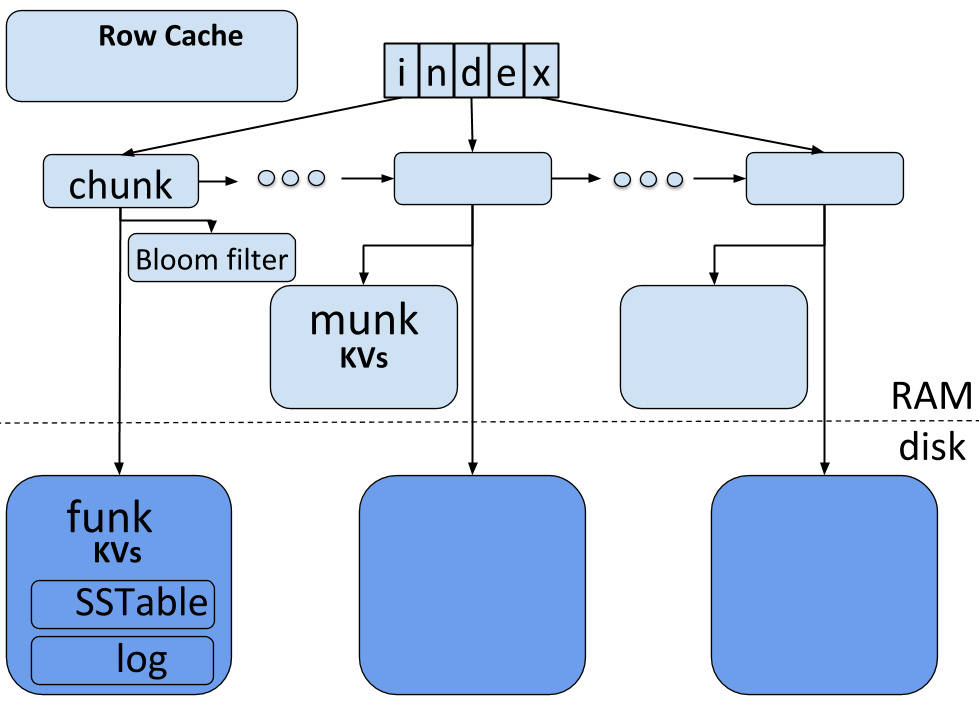
\includegraphics[width=0.75\columnwidth]{PiWi.png}
\caption{\sys: data partitioned by key}
\label{fig:piwi}
\end{subfigure}
%\hspace{1cm}
\begin{subfigure}{0.5\linewidth}\centering
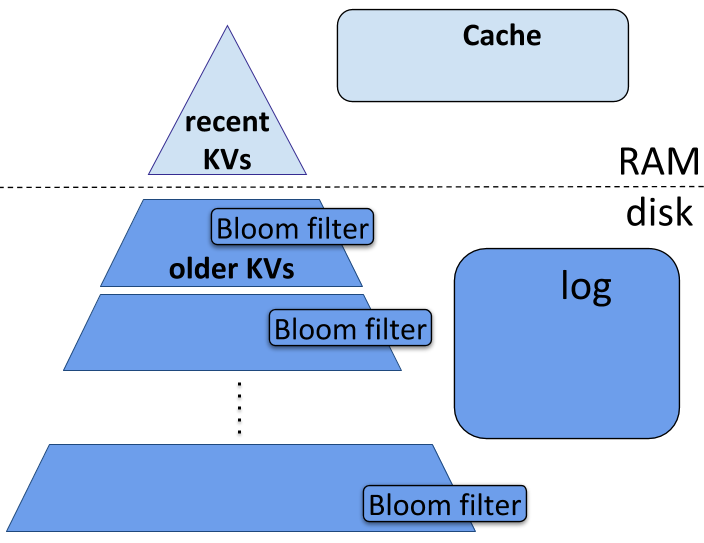
\includegraphics[width=0.75\textwidth]{LSM.png}
\caption{LSM: temporal partitioning}
\label{fig:lsm}
\end{subfigure}
%\hspace{1mm}
%\begin{subfigure}{0.3\linewidth}
%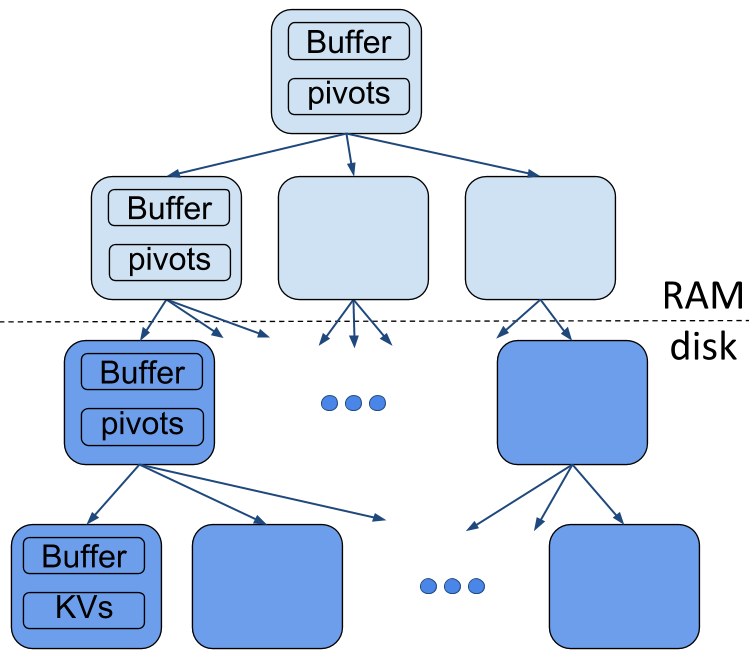
\includegraphics[width=\textwidth]{Bepsilon.png}
%\caption{B$^\epsilon$  tree: data partitioned by key}
%\label{fig:bepsilon}
%\end{subfigure}
%}
\caption{\sys's data layout compared to LSMs trees.}% and B$^\epsilon$ trees.}
\label{fig:layout}
\end{figure*}


%\subsection{Goals}
%\subsection{Guarantees and optimization goals}
\sys\ is a persistent key-value store. Similarly to popular industrial KV-stores~\cite{hbase,leveldb,RocksDB}, 
 it supports concurrent access by multiple threads and ensures 
strong consistency guarantees. 
%\begin{enumerate}\itemsep0pt
%\item 
Specifically its \emph{put, get}, and \emph{range scan} (or scan) operations are \emph{atomic}.  
%For scans, this means that all key-value pairs returned by a single scan belong to a consistent 
%snapshot reflecting the state of the data store at a unique point in time.

Additionally, \sys\ ensures \emph{consistent recovery}: following a crash, the system recovers to a well defined execution 
point some time before the crash. 
When persistence is \emph{asynchronous}, puts are buffered and persisted to disk in the background,  
 trading durability for speed. In this case, some recent updates may be lost but 
 recovery is to a \emph{consistent} state  
in the sense that if some put is lost, then all ensuing (and thus possibly dependent) puts are lost as well.
%\end{enumerate}

Our key design goals are the following:
\begin{enumerate}
\itemsep0pt
\item \emph{Focus on spatial locality.}
 Many NoSQL applications embed multi-dimensional data in a single-dimension composite key. 
 This design provides high spatial locality on the primary dimension (key prefix). We strive
 to express this locality in physical data organization.
 % to exploit it efficiently for scans  by the primary dimension. 
%In addition, a query that retrieves data pertaining to a particular dimension thus needs to atomically 
%retrieve the values pertaining to a range of keys. 
%To favor analytics queries, it is important to optimize such scans. 
 
\item \emph{High performance  with memory-resident working sets.}
To sustain high speed, key-value stores nowadays leverage increasing DRAM sizes 
where they can hold most of the active data set. We strive for maximum performance 
in this ``hyper-local'' case.

\item \emph{Low write amplification.} We seek to minimize disk writes in order to boost performance 
and reduce disk wear, especially for SSD devices. 

\item \emph{Fast recovery.}  Because crashes are inevitable, 
the downtime they entail should be kept  short. 
\end{enumerate}

% Given the aforementioned requirements, we make the following design choices:
%\subsection{Design choices}

Due to lack of space we only discuss high-level design choices and do not go into the low-level design details of the system.

\paragraph{Data organization, compaction, and caching.}
\sys's data organization is illustrated in Figure~\ref{fig:piwi}. 
We organize data, both on-disk and in-memory, in large chunks pertaining to  key ranges.  
Each chunk has a file representation called  \emph{funk} (file chunk), and may be cached in a  memory data structure called \emph{munk} (memory chunk).
This organization exploits spatial locality and is friendly to range scans.

Chunks are organized in a linked list. To speed up key access, 
we index the chunks using a volatile index (a sorted array in our implementation).  
We also partially sort the keys in each chunk for fast in-chunk search.  
 To expedite access to  keys whose chunks are only on-disk  (i.e., have no munks), 
individual popular keys are cached in a \emph{row cache}, 
and \emph{Bloom filters} are used to limit excessive access to disk. 

For comparison, an LSM tree (Figure~\ref{fig:lsm}), organizes data temporally, keeping only the most recent updates in memory.
The in-memory (top level) store optimizes the write-path. To optimize the read path, it uses a large cache.   
For persistence, data is logged to a WAL (write-ahead log). 

 %\emph{In-funk logs and infrequent disk compaction.}
\sys\ logs writes within funks and avoids duplicating the updates  in a separate WAL. This reduces write amplification and expedites recovery. 
The  log is merged into the chunk's sorted key-value table (\emph{SSTable} -- Sorted String Table~\cite{Bigtable2008}) 
via an infrequent background compaction process. 
While a chunk is cached (has a munk), there is no urgency to improve its on-disk organization since 
queries do not access it. Therefore, \sys\ infrequently performs reorganization (compaction) on such funks,
and compacts them only in-memory.
Conversely, when a funk holds cold data, its organization hardly deteriorates, so no compaction is needed.
Note that this is unlike LSM trees, where all disk components are compacted, regardless of which keys reside in memory.
% and whether keys are hot or cold. 

\remove{
A related data organization is that of  B-trees and B$^\epsilon$-trees (Figure~\ref{fig:bepsilon}), who also partition data by key range. 
B$^\epsilon$-trees use in-node update buffers, which resemble \sys's in-funk WALs.
However, their buffers are not used for persistence --- their intent is to amortize the $O(\log n)$ tree traversal cost across multiple updates. 
These trees are analyzed in a model with no memory hierarchy, where all nodes are disk-resident. In practice, their upper layers 
are typically cached in RAM. Given such caching, amortizing the $O(\log n)$ traversal cost is not important, and indeed, practical data stores inspired by
such trees forgo the buffers in internal nodes. Thus, every write entails an in-place update of a leaf node, and every read requires disk access unless the node it reads is cached.
}

 \paragraph{Concurrency and multi-versioning.}
 \sys\ allows high parallelism among threads invoking its API calls. 
 Read operations are wait-free (never block) and puts use lightweight synchronization. 
 To support atomic scans, we  employ a light form of multi-versioning that uses 
copy-on-write to keep old versions only if they may be required by ongoing scans. 
In other words, if a put attempts to overwrite a key required by an active scan, then a new version is created alongside the 
existing one, whereas versions that are not needed by any scan are not retained. 
Thus, version management incurs a low overhead (as it occurs only on scans). 
%It also defines a simple rule for garbage collecting old versions.
In addition, tagging each value with a version allows \sys\ to easily recover to a consistent point in time, namely a version below which all puts have been persisted to disk.

To support atomic scans, production LSM stores employ standard MVCC on top of the LSM tree.  
Each write operation is assigned an auto-incremented sequence number. Since each write adds an additional version to the key it writes to, the memory component often overflows  even if the working set is small enough to fit in memory. This causes frequent data compactions and increases write amplification.
%Like in B-trees 
%Supporting efficient atomic scans in B$^\epsilon$-trees is not trivial, and we are not aware of a published solution addressing atomic scans and persistence with multi-threading in such trees.

%Since updates are buffered in-memory in different paths of the tree before they are persisted in the leaves, supporting consistent recovery in multi-threaded workloads is also not trivial.

